\documentclass[oneside]{book}
\usepackage[backend=biber,natbib=true,style=authoryear]{biblatex}
\addbibresource{/home/hong/1_NQBH/reference/bib.bib}
\usepackage[utf8]{vietnam}
\usepackage{tocloft}
\renewcommand{\cftsecleader}{\cftdotfill{\cftdotsep}}
\usepackage[colorlinks=true,linkcolor=blue,urlcolor=red,citecolor=magenta]{hyperref}
\usepackage{amsmath,amssymb,amsthm,mathtools,float,graphicx,algpseudocode,algorithm,tcolorbox,tikz,tkz-tab}
\DeclareMathOperator{\arccot}{arccot}
\usepackage[inline]{enumitem}
\allowdisplaybreaks
\numberwithin{equation}{section}
\newtheorem{assumption}{Assumption}[section]
\newtheorem{nhanxet}{Nhận xét}[section]
\newtheorem{conjecture}{Conjecture}[section]
\newtheorem{corollary}{Corollary}[section]
\newtheorem{hequa}{Hệ quả}[section]
\newtheorem{definition}{Definition}[section]
\newtheorem{dinhnghia}{Định nghĩa}[section]
\newtheorem{example}{Example}[section]
\newtheorem{vidu}{Ví dụ}[section]
\newtheorem{lemma}{Lemma}[section]
\newtheorem{notation}{Notation}[section]
\newtheorem{principle}{Principle}[section]
\newtheorem{problem}{Problem}[section]
\newtheorem{baitoan}{Bài toán}[section]
\newtheorem{proposition}{Proposition}[section]
\newtheorem{menhde}{Mệnh đề}[section]
\newtheorem{question}{Question}[section]
\newtheorem{cauhoi}{Câu hỏi}[section]
\newtheorem{remark}{Remark}[section]
\newtheorem{luuy}{Lưu ý}[section]
\newtheorem{theorem}{Theorem}[section]
\newtheorem{tiende}{Tiên đề}[section]
\newtheorem{dinhly}{Định lý}[section]
\usepackage[left=0.5in,right=0.5in,top=1.5cm,bottom=1.5cm]{geometry}
\usepackage{fancyhdr}
\pagestyle{fancy}
\fancyhf{}
\lhead{\small \textsc{Sect.} ~\thesection}
\rhead{\small \nouppercase{\leftmark}}
\renewcommand{\sectionmark}[1]{\markboth{#1}{}}
\cfoot{\thepage}
\def\labelitemii{$\circ$}

\title{Some Topics in Elementary Mathematics\texttt{/}Grade 12}
\author{Nguyễn Quản Bá Hồng\footnote{Independent Researcher, Ben Tre City, Vietnam\\e-mail: \texttt{nguyenquanbahong@gmail.com}; website: \url{https://nqbh.github.io}.}}
\date{\today}

\begin{document}
\frontmatter
\maketitle
\setcounter{secnumdepth}{4}
\setcounter{tocdepth}{3}
\tableofcontents
\newpage

%------------------------------------------------------------------------------%

\mainmatter

\part{Đại Số \& Giải Tích -- Algebra \& Analysis}

\chapter{Ứng Dụng Đạo Hàm Để Khảo Sát \& Vẽ Đồ Thị của Hàm Số}

\begin{quotation}
	\textbf{Nội dung.} \textit{Ứng dụng đạo hàm \& giới hạn để xét 1 số tính chất quan trọng của hàm số \& đồ thị như: tính đơn điệu, cực trị, giá trị lớn nhất, giá trị nhỏ nhất của hàm số \& các đường tiệm cận của đồ thị; khảo sát sự biến thiên \& vẽ đồ thị của hàm số của 1 số hàm số đơn giản}.
\end{quotation}

\section{Tính Đơn Điệu của Hàm Số}
\textbf{Nội dung.} \textit{Ứng dụng đạo hàm để xét tính \emph{đơn điệu} (i.e., tính \emph{đồng biến} \& tính \emph{nghịch biến}) của hàm số}.

\begin{dinhnghia}[Hàm số đồng\texttt{/}nghịch biến]
	Giả sử $K$ là 1 khoảng, 1 đoạn hoặc 1 nửa khoảng \& $f$ là hàm số xác định trên $K$. Hàm số $f$ được gọi là \emph{đồng biến} trên $K$ nếu $\forall x_1,x_2\in K$, $x_1 < x_2\Rightarrow f(x_1) < f(x_2)$. Hàm số $f$ được gọi là \emph{nghịch biến} trên $K$ nếu $\forall x_1,x_2\in K$, $x_1 > x_2\Rightarrow f(x_1) < f(x_2)$.
\end{dinhnghia}
I.e., ``nếu hàm số $f$ xác định trên $K$ thì hàm số $f$ đồng biến trên $K$ khi \& chỉ khi với $x\in k$ tùy ý, ta có $\frac{f(x + \Delta x) - f(x)}{\Delta x} > 0$, $\forall\Delta x\ne 0$ mà $x + \Delta x\in K$; hàm số $f$ nghịch biến trên $K$ khi \& chỉ khi với $x\in K$ tùy ý, ta có $\frac{f(x + \Delta x) - f(x)}{\Delta x} < 0$, $\forall\Delta x\ne 0$ mà $x + \Delta x\in K$.'' -- \cite[p. 4]{SGK_Toan_12_giai_tich_nang_cao}

\begin{dinhly}
	Giả sử hàm số $f$ có đạo hàm trên khoảng $I$.
	\begin{enumerate*}
		\item[(a)] Nếu hàm số $f$ đồng biến trên khoảng $I$ thì $f'(x)\ge 0$, $\forall x\in I$.
		\item[(b)] Nếu hàm số $f$ nghịch biến trên khoảng $I$ thì $f'(x)\le 0$, $\forall x\in I$.
	\end{enumerate*}
\end{dinhly}
Đảo lại:

\begin{dinhly}
	\label{thm:dau dao ham & tinh dong bien}
	Giả sử hàm số $f$ có đạo hàm trên khoảng $I$.
	\begin{enumerate*}
		\item[(a)] Nếu $f'(x) > 0$, $\forall x\in I$ thì hàm số $f$ đồng biến trên khoảng $I$.
		\item[(b)] Nếu $f'(x) < 0$, $\forall x\in I$ thì hàm số $f$ nghịch biến trên khoảng $I$.
		\item[(c)] Nếu $f'(x) = 0$, $\forall x\in I$thì hàm số $f$ không đổi trên khoảng $I$.
	\end{enumerate*}
\end{dinhly}
Định lý trên cho ta 1 điều kiện đủ để hàm số đơn điệu trên 1 khoảng.

\begin{luuy}
	Khoảng $I$ trong định lý trên có thể được thay đổi bởi 1 đoạn hoặc 1 nửa khoảng. Khi đó phải bổ sung giả thiết ``Hàm số liên tục trên đoạn hoặc nửa khoảng đó''. E.g.:
	
	\begin{dinhly}
		Nếu hàm số $f$ liên tục trên đoạn $[a;b]$ \& có đạo hàm $f'(x) > 0$ trên khoảng $(a;b)$ thì hàm số $f$ đồng biến trên đoạn $[a;b]$.
	\end{dinhly}
	Người ta thường diễn đạt khẳng định này qua bảng biến thiên như sau:
	
	\begin{center}
		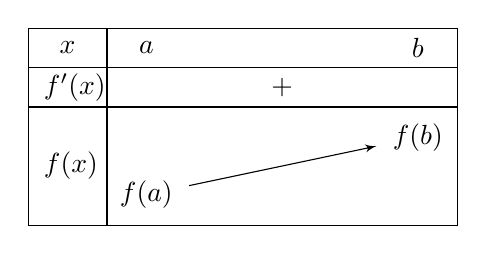
\begin{tikzpicture}
			\tkzTabInit
			[lgt=1,espcl=0.01\linewidth] % tùy chọn
			{$x$/.5, $f’(x)$/.5, $f(x)$/1.5} % cột đầu tiên
			{$a$,$b$} % hàng 1 cột 2
			\tkzTabLine{,+,} % hàng 2 cột 2
			\tkzTabVar{-/ $f(a)$ , +/ $f(b)$} % hàng 3 cột 2
		\end{tikzpicture}
	\end{center}
\end{luuy}
``Việc tìm các khoảng đồng biến \& nghịch biến của 1 hàm số còn được nói gọn là xét \textit{chiều biến thiên của hàm số} đó. Qua định lý đã nêu, ta thấy việc xét chiều biến thiên của 1 hàm số có đạo hàm có thể chuyển về việc xét dấu đạo hàm của nó.'' -- \cite[p. 5]{SGK_Toan_12_giai_tich_nang_cao}

Có thể mở rộng định lý \ref{thm:dau dao ham & tinh dong bien} như sau:

\begin{dinhly}
	Giả sử hàm số $f$ có đạo hàm trên khoảng $I$. Nếu $f'(x)\ge 0$, $\forall x\in I$ (hoặc $f'(x)\le 0$, $\forall x\in I$) \& $f'(x) = 0$ chỉ tại 1 số hữu hạn điểm của $I$ thì hàm số $f$ đồng biến (hoặc nghịch biến) trên $I$.
\end{dinhly}

%------------------------------------------------------------------------------%

\section{Cực Trị của Hàm Số}
\textbf{Nội dung.} \textit{Cực đại, cực tiểu của hàm số; quan hệ giữa cực đại, cực tiểu với dấu của đạo hàm cấp 1 \& đạo hàm cấp 2 của hàm số}.

\subsection{Khái niệm cực trị của hàm số}

%------------------------------------------------------------------------------%

\section{Giá Trị Lớn Nhất \& Giá Trị Nhỏ Nhất của Hàm Số}

%------------------------------------------------------------------------------%

\section{Đồ Thị của Hàm Số \& Phép Tịnh Tiến Hệ Tọa Độ}

%------------------------------------------------------------------------------%

\section{Đường Tiệm Cận của Đồ Thị Hàm Số}

%------------------------------------------------------------------------------%

\section{Khảo Sát Sự Biến Thiên \& Vẽ Đồ Thị của 1 Số Hàm Đa Thức}

%------------------------------------------------------------------------------%

\section{Khảo Sát Sự Biến Thiên \& Vẽ Đồ Thị của 1 Số Hàm Phân Thức Hữu Tỷ}

%------------------------------------------------------------------------------%

\section{1 Số Bài Toán Thường Gặp về Đồ Thị}

%------------------------------------------------------------------------------%

\chapter{Hàm Số Lũy Thừa, Hàm Số Mũ, \& Hàm Số Logarith}

\section{Lũy Thừa với Số Mũ Hữu Tỷ}

%------------------------------------------------------------------------------%

\section{Lũy Thừa với Số Mũ Thực}

%------------------------------------------------------------------------------%

\section{Logarithm}

%------------------------------------------------------------------------------%

\section{Số $\rm e$ \& Logarith Tự Nhiên}

%------------------------------------------------------------------------------%

\section{Hàm Số Mũ \& Hàm Số Logarithm}

%------------------------------------------------------------------------------%

\section{Hàm Số Lũy Thừa}

%------------------------------------------------------------------------------%

\section{Phương Trình Mũ \& Logarithm}

%------------------------------------------------------------------------------%

\section{Hệ Phương Trình Mũ \& Logarithm}

%------------------------------------------------------------------------------%

\section{Bất Phương Trình Mũ \& Logarithm}

%------------------------------------------------------------------------------%

\chapter{Nguyên Hàm, Tích Phân, \& Ứng Dụng}

\section{Nguyên Hàm}

%------------------------------------------------------------------------------%

\section{1 Số Phương Pháp Tìm Nguyên Hàm}

%------------------------------------------------------------------------------%

\section{Tích Phân}

%------------------------------------------------------------------------------%

\section{1 Số Phương Pháp Tính Tích Phân}

%------------------------------------------------------------------------------%

\section{Ứng Dụng Tích Phân Để Tính Diện Tích Hình Phẳng}

%------------------------------------------------------------------------------%

\section{Ứng Dụng Tích Phân Để Tính Thể Tích Vật Thể}

%------------------------------------------------------------------------------%

\chapter{Số Phức}

\section{Số Phức}

%------------------------------------------------------------------------------%

\section{Căn Bậc 2 của Số Phức \& Phương Trình Bậc 2}

%------------------------------------------------------------------------------%

\section{Dạng Lượng Giác của Số Phức \& Ứng Dụng}

%------------------------------------------------------------------------------%

\part{Hình Học -- Geometry}

\chapter{Khối Đa Diện \& Thể Tích của Chúng}

\section{Khái Niệm về Khối Đa Diện}

%------------------------------------------------------------------------------%

\section{Phép Đối Xứng qua Mặt Phẳng \& Sự Bằng Nhau của Các Khối Đa Diện}

%------------------------------------------------------------------------------%

\section{Phép Vị Tự \& Sự Đồng Dạng của Các Khối Đa Diện. Các Khối Đa Diện Đều}

%------------------------------------------------------------------------------%

\section{Thể Tích của Khối Đa Diện}

%------------------------------------------------------------------------------%

\chapter{Mặt Cầu, Mặt Trụ, Mặt Nón}

\section{Mặt Cầu, Khối Cầu}

%------------------------------------------------------------------------------%

\section{Khái Niệm về Mặt Tròn Xoay}

%------------------------------------------------------------------------------%

\section{Mặt Trụ, Hình Trụ, \& Khối Trụ}

%------------------------------------------------------------------------------%

\section{Mặt Nón, Hình Nón, \& Khối Nón}

%------------------------------------------------------------------------------%

\chapter{Phương Pháp Tọa Độ Trong Không Gian}

\section{Hệ Tọa Độ Trong Không Gian}

%------------------------------------------------------------------------------%

\section{Phương Trình Mặt Phẳng}

%------------------------------------------------------------------------------%

\section{Phương Trình Đường Thẳng}

%------------------------------------------------------------------------------%

\printbibliography[heading=bibintoc]
	
\end{document}